\documentclass[11pt,aspectratio=169]{beamer}
\usepackage[italian]{babel}
\usepackage[latin1]{inputenc}
\usepackage{graphicx}
\usepackage{listings}
\usepackage[export]{adjustbox}
% Custom bullets
\usepackage{pifont}
\usepackage[useregional]{datetime2}
\usepackage{tikz}
\usepackage[table]{colortbl}
\usepackage{venndiagram}
\usepackage{amsmath}
\usetikzlibrary{shapes.geometric}
\usetikzlibrary{decorations.markings}
\usetikzlibrary{calc}
\usetikzlibrary{positioning}
\usetikzlibrary{positioning, arrows.meta}

% custom legend
\newcommand{\cbox}[1]{\raisebox{\depth}{\fcolorbox{black}{#1}{\null}}}

\usetheme{Madrid}
\usecolortheme{spruce}

% Redefine labels
\deftranslation[to=Italian]{Section}{Sezione}
\deftranslation[to=Italian]{Subsection}{Sottosezione}


\author[Gianluca Lanchini \and Piermichele Rosati]{Gianluca Lanchini \and Piermichele Rosati}

\institute[]{\large Universit\`a di Camerino\\ \footnotesize Tutorato - Basi di Dati}
\title[Modello Logico dei Dati]{8. Modello Logico dei Dati}
\subtitle{Progettazione Logica, Modello Relazionale, Regole di Derivazione, Dall'E/R al Logico}
\setbeamertemplate{navigation symbols}{}
\setbeamertemplate{section in toc}[sections numbered]
\setbeamertemplate{subsection in toc}[subsections numbered]
%\titlegraphic{
\includegraphics[width=6cm]{img/unicam-logo.jpg}}
\makeatletter
\setbeamertemplate{footline}{
    \leavevmode%
    \hbox{%
        \begin{beamercolorbox}[wd=.333333\paperwidth,ht=2.25ex,dp=1ex,center]{author in head/foot}%
            \usebeamerfont{author in head/foot}\insertshortauthor
        \end{beamercolorbox}%
        \begin{beamercolorbox}[wd=.333333\paperwidth,ht=2.25ex,dp=1ex,center]{title in head/foot}%
            \usebeamerfont{title in head/foot}\insertshorttitle
        \end{beamercolorbox}%
        \begin{beamercolorbox}[wd=.333333\paperwidth,ht=2.25ex,dp=1ex,right]{date in head/foot}%
            \usebeamerfont{date in head/foot}\today\hspace*{5 em}
            \insertframenumber{} / \inserttotalframenumber\hspace*{2ex} 
        \end{beamercolorbox}%
    }%
    \vskip0pt%
}
\makeatother


\AtBeginSection[]
{
\begin{frame}<beamer>
\frametitle{Indice}
\tableofcontents[currentsection]
\end{frame}
}

\begin{document}
\begin{frame}
\centering

\includegraphics[width=5.5cm]{../img/unicam-logo.jpg}
\date{\today}
\titlepage
\end{frame}
\addtobeamertemplate{frametitle}{}{%
\begin{tikzpicture}[remember picture,overlay]
\node[anchor=north east,yshift=2pt] at (current page.north east) {
\includegraphics[height=2cm]{../img/unicam-logo-notext.png}};
\end{tikzpicture}}

%\begin{frame}
%\titlepage
%\end{frame}

\section{Concetti fondamentali del Modello Relazionale}
\def\cartesianproductAOneATwo{
    \begin{tikzpicture}
        \node[circle, draw, minimum size=5cm, label=above:{$A_1 \times A_2$}] (set1) at (0,0) {};
        \node at (0,1.5) (P1) {(4,3)};
        \node at (-1,0.5) (P2) {(9,2)};
        \node at (1.5,1) (P3) {(4,2)};
        \node at (1,0) (P4) {(9,3)};
        \node at (-1.5,-0.5) (P5) {(16,2)};
        \node at (-0.5,-1.25) (P6) {(16,3)};
    \end{tikzpicture}
}
\def\cartesianproductRedQ{
    \begin{tikzpicture}
        \node[circle, draw, minimum size=5cm, label=above:{$A_1 \times A_2$}] (set1) at (0,0) {};
        \node at (0,1.5) (P1) {(4,3)};
        \node at (-1,0.5) (P2) {(9,2)};
        \node at (1.5,1) (P3) {(4,2)};
        \node at (1,0) (P4) {(9,3)};
        \node at (-1.5,-0.5) (P5) {(16,2)};
        \node at (-0.5,-1.25) (P6) {(16,3)};
    
        % Dashed red circle around P3 and P4
        \node[circle, draw=red, dashed, minimum size=2cm, label=above:{\textcolor{red}{Q}}] at (1.25,0.5) {};
    \end{tikzpicture}
}
\def\AutomobiliRelationship{
    $Automobili$
        
        \begin{tabular}{|c|c|c|c|c|}
            \hline
            \rowcolor{cyan!30}$Modello$ & $Costruttore$ & $Segmento$ & $Porte$ & $Posti$ \\
            \hline
            Serie 3 & BMW & D & 4 & 5 \\ \hline
            Panda & Fiat & B & 5 & 4 \\ \hline
            Giulietta & Alfa Romeo & C & 5 & 5 \\ \hline
            Bravo & Fiat & C & 5 & 5 \\ \hline
            Punto & Fiat & B & 3 & 5 \\ \hline
            C3 & Citroen & B & 5 & 5 \\ \hline
            C4 & Citroen & C & 5 & 5 \\ \hline
            Delta & Lancia & C & 5 & 5 \\ \hline
        \end{tabular}
}
\begin{frame}{Concetti fondamentali del Modello Relazionale}
Lo sviluppo di un database di un sistema informativo passa attraverso diverse fasi di progettazione, o livelli:
\begin{itemize}[<+->]
    \item livello concettuale;
    \item livello logico;
    \item livello fisico.
\end{itemize}
\pause
\begin{block}{Modello Relazionale}
Il \textbf{modello relazionale} \`e il modello pi\`u utilizzato per la progettazione di basi di dati.
\pause
\newline
\\ In questo modello una base di dati \`e vista come un insieme di tabelle sulle quali possono essere eseguite opportune operazioni.
\pause
\begin{itemize}[<+->]
    \item Il modello \`e chiamato relazionale perch\`e \`e fondato sul concetto matematico di \textbf{relazione} tra insiemi di oggetti.
    \item Esso \`e un modello fondato sui valori.
\end{itemize}
\end{block}
\end{frame}
%
\begin{frame}{Il concetto di Relazione}
Per capire il concetto di relazione e comprendere come si possa rappresentare una relazione mediante tabelle, consideriamo un semplice esempio.

\pause
Consideriamo i 2 insiemi $A_1 = \{4, 9, 16\}$ e $A_2 = \{2, 3\}$.
\pause
\begin{center}
    \begin{tikzpicture}
        \node[circle, draw, minimum size=3.5cm, label=above:{$A_1$}] (set1) at (0,0) {};
        % Label the points in the first set
        \node at (-1,1) (P1) {4};
        \node at (0,0.5) (P2) {9};
        \node at (1,-1) (P3) {16};
    
        \node[circle, draw, minimum size=3.5cm, label=above:{$A_2$}] (set2) at (6,0) {};
        % Label the points in the second set
        \node at (5,1) (A1) {2};
        \node at (6,0.5) (A2) {3};
    \end{tikzpicture}
\end{center}
\end{frame}
%
\begin{frame}{Il concetto di Relazione}
\begin{minipage}[t]{0.4\linewidth}
Prodotto cartesiano tra $A_1$ e $A_2$:
\pause
\begin{center}
\cartesianproductAOneATwo
\end{center}
\end{minipage}%
\hfill%
\begin{minipage}[t]{0.6\linewidth}
\begin{block}{Prodotto cartesiano}
Il \textbf{prodotto cartesiano} di $A_1$ e $A_2$ si indica con $A_1 \times A_2$ ed \`e formato dall'insieme delle coppie $(x,y)$ dove $x$ appartiene ad $A_1$ e $y$ appartiene ad $A_2$.
\end{block}
\end{minipage}
\end{frame}
%
\begin{frame}{Il concetto di Relazione}
\begin{minipage}[t]{0.4\linewidth}
Prodotto cartesiano tra $A_1$ e $A_2$:
\begin{center}
\cartesianproductRedQ
\end{center}
\end{minipage}%
\hfill%
\begin{minipage}[t]{0.6\linewidth}
\begin{block}{Coppie significative}
Alcune coppie del prodotto cartesiano sembrano essere pi\`u significative di altre.
\pause
\\Come per il sottoinsieme $Q$, composo dalle coppie di valori $(x,y)$ dove $x$ \`e il quadrato di $y$.
\pause
\newline
\\ $Q$ pu\`o essere descritto da: ``$x$ \`e il quadrato di $y$'', che esprime la relazione esistente tra $x$ e $y$.
{\scriptsize \[ Q = {(4,2),(9,3)} \subseteq A_1 \times A_2 = {(4,2),(4,3),(9,2),(9,3),(16,2),(16,3)} \]}
\end{block}
\end{minipage}
\end{frame}
%
\begin{frame}{Il concetto di Relazione}
\begin{minipage}[t]{0.4\linewidth}
Prodotto cartesiano tra $A_1$ e $A_2$:
\begin{center}
\cartesianproductRedQ
\end{center}
\end{minipage}%
\hfill%
\begin{minipage}[t]{0.6\linewidth}
\begin{block}{Relazione}
Si dice \textbf{relazione} su due insiemi $A_1$ e $A_2$ un sottoinsieme $R$ del prodotto cartesiano $A_1 \times A_2$.
\end{block}
\pause
\begin{itemize}[<+->]
    \item $Q$ \`e la relazione \textit{QuadratoDi};
    \item Sia $A_1 \times A_2$ che la relazione $Q$, possono essere rappresentate con tabelle!
    \item Ogni tabella \`e composta da tante righe quante sono gli elementi del prodotto cartesiano oppure \textit{QuadratoDi} e da 2 colonne, per rappresentare, ordinatamente, il valore del primo e del secondo elemento delle coppie $(x,y)$.
\end{itemize}
\end{minipage}
\end{frame}
%
\begin{frame}{Il concetto di Relazione}
\begin{minipage}[t]{0.4\linewidth}
\begin{center}
\cartesianproductRedQ
\end{center}
\end{minipage}%
\hfill%
\begin{minipage}[t]{0.6\linewidth}
\vspace{-5cm}
\begin{center}
    \begin{minipage}{0.4\textwidth}
        \begin{center}
            $A_1 \times A_2$
            
            \pause
            \begin{tabular}{|c|c|}
                \hline
                \rowcolor{cyan!30}$A_1$ & $A_2$ \\
                \hline
                4 & 2 \\ \hline
                4 & 3 \\ \hline
                9 & 2 \\ \hline
                9 & 3 \\ \hline
                16 & 2 \\ \hline
                16 & 3 \\ \hline
            \end{tabular}
        \end{center}
    \end{minipage}
    \hspace{1cm}
    \begin{minipage}{0.4\textwidth}
        \begin{center}
            \pause
            \textit{QuadratoDi}
            \pause
            \begin{tabular}{|c|c|}
                \hline
                \rowcolor{cyan!30}$A_1$ & $A_2$ \\
                \hline
                4 & 2 \\ \hline
                9 & 3 \\ \hline
            \end{tabular}
        \end{center}
    \end{minipage}
\end{center}
\end{minipage}
\end{frame}
%
\begin{frame}{Un esempio concreto di Relazione}
\begin{minipage}{0.9\textwidth}
    Riferendoci al mondo dell'automobile, consideriamo gli insiemi \textit{Modello} e \textit{Costruttore}, cos\`i definiti:
\end{minipage}
\vspace{-.3cm}
\pause
\[ Modello = \{Panda, Cinquecento, C3, C4\}\]
\[ Costruttore = \{Citroen, Fiat\} \]
\begin{minipage}[t]{0.48\linewidth}
\pause
    \begin{center}
        $Modello \times Costruttore$
        
        \pause
        \begin{tabular}{|c|c|}
            \hline
            \rowcolor{cyan!30}$Modello$ & $Costruttore$ \\
            \hline
            Panda & Citroen \\ \hline
            Cinquecento & Citroen \\ \hline
            C3 & Citroen \\ \hline
            C4 & Citroen \\ \hline
            Panda & Fiat \\ \hline
            Cinquecento & Fiat \\ \hline
            C3 & Fiat \\ \hline
            C4 & Fiat \\ \hline
        \end{tabular}
    \end{center}
\end{minipage}%
\hfill%
\begin{minipage}[t]{0.48\linewidth}
    \begin{center}
        \pause
        \textit{ProdottoDa}

        \pause
        \begin{tabular}{|c|c|}
            \hline
            \rowcolor{cyan!30}$Modello$ & $Costruttore$ \\
            \hline
            C3 & Citroen \\ \hline
            C4 & Citroen \\ \hline
            Panda & Fiat \\ \hline
            Cinquecento & Fiat \\ \hline
        \end{tabular}
    \end{center}
\pause
\vspace{-.55cm}
\begin{block}{Nota bene}
    {\small Questo sottoinsieme formato dai 4 elementi di $Modello \times Costruttore$ \`e indicato, \textbf{in modo significativo}, come \textit{ProdottoDa}.}
\end{block}
\end{minipage}
\end{frame}
%
\begin{frame}{Relazione}
Pi\`u in generale:
\begin{block}{Relazione}
Una \textbf{relazione} su $n$ insiemi $A_1, A_2, \ldots, A_n$ \`e un sottoinsieme dell'insieme di tutte le $n$-uple $a_1, a_2, \ldots, a_n$ che si possono costruire prendendo nell'ordine un elemento $a_1$ dal primo insieme $A_1$, $a_2$ dal secondo insieme $A_2$, e cos\`i via.
\pause
\begin{itemize}[<+->]
    \item Una relazione con $n$-colonne si indica come una relazione di \textbf{grado} $n$;
    \item Il nome con il quale si identifica una colonna si chiama \textbf{attributo}.
    \item L'insieme dei valori che possono essere assunti da un attributo definisce il \textbf{dominio} di quell'attributo.
    \item Il numero delle $n$-uple (anche dette tuple) che compongono la tabella si chiama \textbf{cardinalit\`a} della relazione.
\end{itemize}
\end{block}
\end{frame}
%
\begin{frame}{Esempio: grado, cardinalit\`a, attributi e dominio}
\vspace{-.7cm}
\begin{minipage}[t]{0.48\linewidth}
    \begin{center}
        $Modello \times Costruttore$
        
        \begin{tabular}{|c|c|}
            \hline
            \rowcolor{cyan!30}$Modello$ & $Costruttore$ \\
            \hline
            Panda & Citroen \\ \hline
            Cinquecento & Citroen \\ \hline
            C3 & Citroen \\ \hline
            C4 & Citroen \\ \hline
            Panda & Fiat \\ \hline
            Cinquecento & Fiat \\ \hline
            C3 & Fiat \\ \hline
            C4 & Fiat \\ \hline
        \end{tabular}
    \end{center}
\end{minipage}%
\hfill%
\begin{minipage}[t]{0.5\linewidth}
    \begin{center}
        \textit{ProdottoDa}

        \begin{tabular}{|c|c|}
            \hline
            \rowcolor{cyan!30}$Modello$ & $Costruttore$ \\
            \hline
            C3 & Citroen \\ \hline
            C4 & Citroen \\ \hline
            Panda & Fiat \\ \hline
            Cinquecento & Fiat \\ \hline
        \end{tabular}
    \end{center}
\pause
La relazione \textit{ProdottoDa}:
\begin{itemize}
    \item \`e una relazione di \textbf{grado}: \pause 2;
    \item \`e una relazione di \textbf{cardinalit\`a}: \pause 4.
    \item La coppia (Panda, Fiat) \`e una delle 4 tuple della relazione.
\end{itemize}
\end{minipage}
\pause

\vspace{.5cm}
La relazione ha due \textbf{attributi}: \textit{Modello} e \textit{Costruttore} che assumono valori nei 2 domini, formati, rispettivamente, dall'insieme dei modelli di automobili prodotte e dall'insieme dei costruttori di automobili.
\end{frame}
%
\begin{frame}{Esempio: una relazione pi\`u complessa}
\begin{minipage}[t]{0.6\linewidth}
    \begin{center}
        \AutomobiliRelationship
    \end{center}
\end{minipage}%
\hfill%
\begin{minipage}[t]{0.4\linewidth}
\begin{center}
    \begin{itemize}[<+->]
        \item La relazione (o tabella) \textbf{Automobili} rappresenta un'entit\`a;
        \item Ogni $n$-upla rappresenta un'istanza dell'entit\`a;
        \item Le colonne contengono i valori assunti degli attributi dell'entit\`a.
        \item \textbf{Cardinalit\`a}: \pause {8 (numero di tuple/righe/record della tabella);}
        \item \textbf{Grado}: \pause {5 (numero di attributi/colonne/campi della tabella)}.
    \end{itemize}
\end{center}
\end{minipage}
\end{frame}
%
\begin{frame}{Relazioni e chiavi}
\vspace{-.9cm}
\begin{center}
    \AutomobiliRelationship
\end{center}
\pause

L'attributo \textit{Modello} \`e \textbf{chiave} di \textit{Automobili}.

\pause
\begin{block}{Chiave}
    La \textbf{chiave} della relazione \`e un attributo (o una combinazione minimale di attributi) che identifica univocamente le $n$-uple della relazione, cio\`e ogni riga della tabella possiede valori diversi per l'attributo (o gli attributi) chiave.
\end{block}
\end{frame}
%
\begin{frame}{Relazioni e chiavi}
La chiave (formata da uno o pi\`u attributi) identifica la $n$-upla all'interno della tabella:
\pause

per questo motivo il modello relazionale fissa una regola di integrit\`a sui dati, detta\\ \textbf{integrit\`a sull'entit\`a} (entity integrity), secondo cui la chiave primaria non pu\`o avere valore nullo.
\end{frame}
%
\begin{frame}{Rappresentare le tabelle}
Una tabella si rappresenta mediante il suo \textbf{schema}, secondo una struttura del tipo:
\[ \textbf{nomeTabella}(\underline{campoChiave}, campo1, campo2, \ldots, campoN) \]
\pause

identificando tra parentesi, dopo il nome della relazione:
\pause
\begin{itemize}[<+->]
    \item i nomi degli attributi separati dalla virgola;
    \item e sottolineando l'attributo chiave.
\end{itemize}
\pause

\[ \textbf{Automobili}(\underline{Modello}, Costruttore, Segmento, Porte, Posti) \]
\end{frame}
%
\begin{frame}{Rappresentare le tabelle}
Lo \textbf{schema di un database relazionale} \`e definito dallo schema delle tabelle che lo compongono.

\pause

Per esempio, il database con le vendite di prodotti che appartengono a diversi reparti di un negozio, ha il seguente schema:
\[ \textbf{Reparti}(\underline{CodReparto}, NomeReparto) \]
\[ \textbf{Prodotti}(\underline{CodProdotto}, Descrizione, Prezzo, CodReparto) \]
\[ \textbf{Vendite}(\underline{Numero}, Data, Quantita, CodProdotto) \]
\end{frame}
%
\section{La derivazione delle relazioni dal Modello E/R}
\def\ERDipendenteAutoAziendale{
    \begin{tikzpicture}[remember picture]
        % Define styles for shapes
        \tikzstyle{rectangle} = [draw, minimum width=3cm, minimum height=1cm]
        \tikzstyle{rhombus} = [draw, diamond, minimum width=3cm, minimum height=1cm, aspect=2]
        % Draw shapes
        \node[rectangle] (rect1) at (1.5, -1) {
            \scriptsize
                \begin{tabular}{c}
                    \textbf{Dipendente} \\
                    \hline
                    Matricola \{PK\} \\
                    Cognome \\
                    Nome \\
                    DataNascita \\
                    LuogoNascita \\
                \end{tabular}
        };
        \node[rhombus] (rhombus) at (7, -1) {\scriptsize EssereAssegnata};
        \node[rectangle] (rect2) at (12.5, -1) {
            \scriptsize
                \begin{tabular}{c}
                    \textbf{AutoAziendale} \\
                    \hline
                    Targa \{PK\} \\
                    Modello \\
                    Costruttore \\
                    Cilindrata \\
                \end{tabular}
            };

        % Draw arrows
        \draw (rect1) -- (rhombus) node[midway, above] {(0,1)};
        \draw (rhombus) -- (rect2) node[midway, above] {(1,1)};
    \end{tikzpicture}
}
\begin{frame}{La derivazione delle relazioni dal modello E/R}
Dal modello concettuale dei dati \`e possibile ottenere il \textbf{modello logico} dei dati.

\pause
In altre parole si pu\`o definire la struttura degli archivi adatti per organizzare i dati.

\pause
Nel caso del modello relazionale le tabelle, che costituiscono il modello logico, vengono ricavate dal modello E/R mediante alcune semplici \textbf{regole di derivazione}.
\end{frame}
%
\begin{frame}[allowframebreaks]{Le regole di derivazione}
\begin{enumerate}
    \item Ogni entit\`a diventa una relazione.
    \item Ogni attributo di un'entit\`a diventa un attributo della relazione, cio\`e il nome di una colonna della tabella.
    \item Ogni attributo della relazione eredita le caratteristiche dell'attributo dell'entit\`a da cui deriva.
    \item L'identificatore univoco di un'entit\`a diventa la \textit{chiave primaria} della relazione derivata.
    \item L'associazione \textit{uno a uno} diventa un'unica relazione che contiene gli attributi della prima e della seconda entit\`a.
    \item L'associazione \textit{uno a molti} viene rappresentata aggiungendo, agli attributi dell'entit\`a che svolge il ruolo a molti, l'identificatore univoco dell'entit\`a che svolge il ruolo a uno nell'associazione. Questo identificatore che prende il nome di \textbf{chiave esterna} (foreign key) dell'entit\`a associata, \`e costituito dll'insieme di attributi che compongono la chiave dell'entit\`a a uno dell'assocazione. Gli eventuali attributi dell'associazione vengono inseriti nella relazione che rappresenta l'entit\`a a molti, assieme alla chiave esterna.
    \item L'associazione \textit{molti a molti} diventa una nuova relazione composta dagli identificatori univoci delle due entit\`a e dagli eventuali attributi che compongono le chiavi delle 2 entit\`a.
\end{enumerate}
\end{frame}
%
\begin{frame}{Suggerimenti}
\begin{itemize}[<+->]
    \item Applicare le regole di derivazione in modo sistematico;
    \item Sottolineare la \underline{chiave primaria};
    \item Aggiungere simboli come $^*$ o $^\#$ per indicare la presenza di chiavi esterne: $chiaveEsterna1^*$, $chiaveEsterna2^\#$ \ldots;
    \item Convertire i nomi delle entit\`a al plurale, per rappresentare il fatto che la relazione contiene l'insieme delle tuple che sono le istanze delle entit\`a.
\end{itemize}
\end{frame}
%
\begin{frame}{Regole di derivazione: Associazioni 1 a 1}
\begin{center}
    \begin{tikzpicture}[remember picture]
        % Define styles for shapes
        \tikzstyle{rectangle} = [draw, minimum width=3cm, minimum height=1cm]
        \tikzstyle{rhombus} = [draw, diamond, minimum width=3cm, minimum height=1cm, aspect=2]
        % Draw shapes
        \node[rectangle] (rect1) at (1.5, -1) {
                \begin{tabular}{c}
                    \textbf{Cittadino} \\
                    \hline
                    CodiceFiscale \{PK\} \\
                    Cognome \\
                    Nome \\
                    DataNascita \\
                    LuogoNascita \\
                \end{tabular}
        };
        \node[rhombus] (rhombus) at (7, -1) {EssereAssegnato};
        \node[rectangle] (rect2) at (12.5, -1) {
                \begin{tabular}{c}
                    \textbf{CodiceSSN} \\
                    \hline
                    CodiceSanitario \{PK\} \\
                    NumeroAsl \\
                    CodRegione \\
                \end{tabular}
            };

        % Draw arrows
        \draw (rect1) -- (rhombus) node[midway, above] {(1,1)};
        \draw (rhombus) -- (rect2) node[midway, above] {(1,1)};
    \end{tikzpicture}
\end{center}
\pause

Applicando le regole di derivazione, si ricava la tabella \textbf{Anagrafe} con gli attributi di entrambe le entit\`a:

\textbf{Anagrafe}(\underline{CodiceFiscale}, Cognome, Nome, DataNascita, LuogoNascita, CodiceSanitario, NumeroAsl, CodRegione)
\end{frame}
%
\begin{frame}{Regole di derivazione: Associazioni 1 a 1}
\begin{minipage}{0.9\textwidth}
Consideriamo l'associazione tra \textit{Dipendente} e \textit{AutoAziendale} nel caso di un'azienda dove, come avviene nella maggior parte dei casi, solo a una piccola parte dei dipendenti \`e assegnata un'auto aziendale.
\end{minipage}
\pause
\begin{center}
\ERDipendenteAutoAziendale
\end{center}
\pause

Applicando le regola di derivazione 5, si ricava la seguente tabella:
\pause

\textbf{Dipendenti}(\underline{Matricola}$^*$, Cognome, Nome, DataNascita, LuogoNascita, Targa, Modello, Costruttore, Cilindrata)
\pause

\`E corretto modellare in questo modo l'associazione tra \textit{Dipendente} e \textit{AutoAziendale}?
\pause

S\`i, ma poich\`e solo una piccola parte dei dipendenti ha un'auto aziendale, la maggior parte dei valori degli attributi \textit{Targa}, \textit{Modello}, \textit{Costruttore} e \textit{Cilindrata} saranno \textit{NULL}.
\end{frame}
%
\begin{frame}{Regole di derivazione: Associazioni 1 a 1}
In alcune situazioni \`e preferibile trattare le associazioni uno a uno in altro modo e modellarle come se fossero uno a molti:
\pause
\begin{center}
\ERDipendenteAutoAziendale
\end{center}
\pause

Applicando le regola di derivazione 6 al posto della 5, (Dipendente: uno, AutoAziendale: molti) si ricavano le seguenti tabelle:
\pause

\textbf{Dipendenti}(\underline{Matricola}$^*$, Cognome, Nome, DataNascita, LuogoNascita)
\pause

\textbf{AutoAziendali}(\underline{Targa}, Modello, Costruttore, Cilindrata, Matricola$^*$)
\end{frame}
%
\begin{frame}{Regole di derivazione: Associazioni 1 a N}
\begin{center}
    \begin{tikzpicture}[remember picture]
        % Define styles for shapes
        \tikzstyle{rectangle} = [draw, minimum width=3cm, minimum height=1cm]
        \tikzstyle{rhombus} = [draw, diamond, minimum width=3cm, minimum height=1cm, aspect=2]
        % Draw shapes
        \node[rectangle] (rect1) at (1.5, -1) {
                \begin{tabular}{c}
                    \textbf{Contratto} \\
                    \hline
                    Codice \{PK\} \\
                    Descrizione \\
                    StipendioBase \\
                    DataScadenza \\
                \end{tabular}
        };
        \node[rhombus] (rhombus) at (7, -1) {Applicare};
        \node[rectangle] (rect2) at (12.5, -1) {
                \begin{tabular}{c}
                    \textbf{Dipendente} \\
                    \hline
                    Matricola \{PK\} \\
                    Cognome \\
                    Nome \\
                    Indirizzo \\
                    Qualifica \\
                \end{tabular}
            };

        % Draw arrows
        \draw (rect1) -- (rhombus) node[midway, above] {(0,N)};
        \draw (rhombus) -- (rect2) node[midway, above] {(1,1)};
    \end{tikzpicture}
\end{center}
\pause

Applicando le regole di derivazione, si ricavano le seguenti tabelle:

\textbf{Contratti}(\underline{Codice}$^*$, Descrizione, StipendioBase, DataScadenza)
\pause

\textbf{Dipendenti}(\underline{Matricola}, Cognome, Nome, Indirizzo, Qualifica, CodiceContratto$^*$)

\pause
\vspace{.1cm}

Agli attributi di \textit{Dipendenti} (a molti) \`e aggiunta come chiave esterna \textit{CodiceContratto}, in corrispondenza della chiave primaria della tabella \textit{Contratti} (a uno).
\end{frame}
%
\begin{frame}{Regole di derivazione: Associazioni 1 a N con attributi}
\begin{center}
    \begin{tikzpicture}[remember picture]
        % Define styles for shapes
        \tikzstyle{rectangle} = [draw, minimum width=2cm, minimum height=1cm]
        \tikzstyle{rhombus} = [draw, diamond, minimum width=2cm, minimum height=1cm, aspect=2]
        % Draw shapes
        \node[rectangle] (rect1) at (1.5, -1) {
            \scriptsize
                \begin{tabular}{c}
                    \textbf{Persona} \\
                    \hline
                    CodiceFiscale \{PK\} \\
                    Cognome \\
                    Nome \\
                    DataNascita \\
                    Indirizzo \\
                \end{tabular}
        };
        \node[rhombus] (rhombus) at (7, -1) {\scriptsize Acquistare};
        \node[rectangle] (rect2) at (11.5, -1) {
            \scriptsize
                \begin{tabular}{c}
                    \textbf{Automobile} \\
                    \hline
                    Targa \{PK\} \\
                    Modello \\
                    Costruttore \\
                    Cilindrata \\
                    PrezzoListino \\
                \end{tabular}
            };
        % Acquistare rectangle under the rhombus
        \node[rectangle] (rect3) at (7, -3) {
            \scriptsize
            \begin{tabular}{c}
                 \\
                \hline
                Data \\
                Prezzo \\
            \end{tabular}
        };

        % Draw arrows
        \draw (rect1) -- (rhombus) node[midway, above] {(0,N)};
        \draw (rhombus) -- (rect2) node[midway, above] {(1,1)};
        % line from rhombus to the Fornire rectangle
        \draw (rhombus) -- (rect3) node[midway, right] {};
    \end{tikzpicture}
\end{center}
\pause

Applicando le regole di derivazione, si ricavano le seguenti tabelle:

\pause

\textbf{Persone}(\underline{CodiceFiscale}, Cognome, Nome, DataNascita, Indirizzo)
\pause

\textbf{Automobili}(\underline{Targa}, Modello, Costruttore, Cilindrata, PrezzoListino, CodiceFiscale$^*$, Data, Prezzo)

\pause
\vspace{.1cm}

Nella tabella \textit{Automobili} agli attributi di \textit{Automobile}, sono aggiunti: la chiave esterna, CodiceFiscale e gli attributi che fanno parte dell'associazione \textit{Acquistare}.
\end{frame}
%
\begin{frame}{Regole di derivazione: Associazioni N a N con attributi}
\begin{center}
    \begin{tikzpicture}[remember picture]
        % Define styles for shapes
        \tikzstyle{rectangle} = [draw, minimum width=2cm, minimum height=1cm]
        \tikzstyle{rhombus} = [draw, diamond, minimum width=2cm, minimum height=1cm, aspect=2]
        % Draw shapes
        \node[rectangle] (rect1) at (1.5, -1) {
            \scriptsize
                \begin{tabular}{c}
                    \textbf{Docente} \\
                    \hline
                    CodiceDocente \{PK\} \\
                    Cognome \\
                    Nome \\
                    Qualifica \\
                    Materia \\
                \end{tabular}
        };
        \node[rhombus] (rhombus) at (7, -1) {\scriptsize Insegnare};
        \node[rectangle] (rect2) at (11, -1) {
            \scriptsize
                \begin{tabular}{c}
                    \textbf{Classe} \\
                    \hline
                    SiglaClasse \{PK\} \\
                    NumeroAlunni \\
                    Aula \\
                \end{tabular}
            };
        % Acquistare rectangle under the rhombus
        \node[rectangle] (rect3) at (7, -3) {
            \scriptsize
            \begin{tabular}{c}
                 \\
                \hline
                NumeroOre \\
            \end{tabular}
        };

        % Draw arrows
        \draw (rect1) -- (rhombus) node[midway, above] {(0,N)};
        \draw (rhombus) -- (rect2) node[midway, above] {(1,N)};
        % line from rhombus to the Fornire rectangle
        \draw (rhombus) -- (rect3) node[midway, right] {};
    \end{tikzpicture}
\end{center}
\pause

Applicando le regole di derivazione, si ricavano le seguenti tabelle:

\pause

\textbf{Docenti}(\underline{CodiceDocente}$^*$, Cognome, Nome, Qualifica, Materia)
\pause

\textbf{Classi}(\underline{SiglaClasse}$^\#$, NumeroAlunni, Aula)

\pause

\textbf{Insegnare}(\underline{CodiceDocente}$^*$, \underline{SiglaClasse}$^\#$, NumeroOre)

\pause
La tabella \textit{Insegnare} contiene le chiavi esterne delle tabelle \textit{Docenti} e \textit{Classi} e l'attributo NumeroOre che fa parte dell'associazione \textit{Insegnare}.
\end{frame}
%
\begin{frame}{Regole di derivazione: Dettagli su Associazioni 1 a 1}
\begin{minipage}{0.9\textwidth}
Ogni classe deve avere uno e un solo coordinatore, un docente coordinare una sola classe, ma ci sono docenti che non sono coordinatori.
\end{minipage}
\begin{center}
    \begin{tikzpicture}[remember picture]
        % Define styles for shapes
        \tikzstyle{rectangle} = [draw, minimum width=2cm, minimum height=1cm]
        \tikzstyle{rhombus} = [draw, diamond, minimum width=2cm, minimum height=1cm, aspect=2]
        % Draw shapes
        \node[rectangle] (rect1) at (1.5, -1) {
            \scriptsize
                \begin{tabular}{c}
                    \textbf{Docente} \\
                    \hline
                    CodiceDocente \{PK\} \\
                    Cognome \\
                    Nome \\
                    Qualifica \\
                    Materia \\
                \end{tabular}
        };
        \node[rhombus] (rhombus) at (7, -1) {\scriptsize Coordinare};
        \node[rectangle] (rect2) at (11, -1) {
            \scriptsize
                \begin{tabular}{c}
                    \textbf{Classe} \\
                    \hline
                    SiglaClasse \{PK\} \\
                    NumeroAlunni \\
                    Aula \\
                \end{tabular}
            };

        % Draw arrows
        \draw (rect1) -- (rhombus) node[midway, above] {(0,1)};
        \draw (rhombus) -- (rect2) node[midway, above] {(1,1)};
    \end{tikzpicture}
\end{center}
\vspace{-.4cm}
\pause

Applicando le regole di derivazione, si ricaverebbe una sola tabella dove comparirebbero molte righe con valori NULL per i docenti che non sono coordinatori.

\pause

Meglio trattare l'associazione come 1 a N, con \textit{Classe} che gioca il ruolo a molti:

\pause

\textbf{Classi}(\underline{SiglaClasse}, NumeroAlunni, Aula, Coordinatore$^*$)

\pause

\textbf{Docenti}(\underline{CodiceDocente}$^*$, Cognome, Nome, Qualifica, Materia)

\pause

Nel caso di partecipazione facoltativa di entrambe le entit\`a \`e indifferente  la scelta dell'entit\`a che gioca il ruolo a molti.
\end{frame}
%
\begin{frame}{Regole di derivazione: Dettagli su Associazioni ricorsive}
\vspace{-.5cm}
\begin{minipage}{0.9\textwidth}
\textit{Coordinare} \`e un'associazione ricorsiva uno a molti tra i dipendenti di un'impresa: alcuni dipendenti sono anche supervisori e coordinano un certo numero di persone. I dipendenti coordinati (collaboratori) dipendono da un solo supervisore, ma ci sono dipendenti che non dipendono da alcun supervisore.
\end{minipage}

\begin{center}
    \begin{tikzpicture}
        % Define styles for shapes
        \tikzset{
            rectangle/.style={draw, minimum width=3cm, minimum height=1cm},
            rhombus/.style={draw, diamond, minimum width=3cm, minimum height=1cm, aspect=2}
        }
        % Draw shapes
        \node[rectangle] (rect1) at (2, -0.5) {
            \scriptsize
                \begin{tabular}{c}
                    \textbf{Dipendente} \\
                    \hline
                    Matricola \{PK\} \\
                    Cognome \\
                    Nome \\
                    DataNascita \\
                    LuogoNascita \\
                \end{tabular}
        };

        \node[rhombus] (rhombus) at (7, -0.5) {\scriptsize Coordinare};
        % Draw arrows
        \draw[-] (rect1) -- (rhombus) node[midway, above] {};
        \draw[-] (rhombus) -- (rect1) node[midway, below] {};
        % Additional arrows
        \draw[-] (rhombus) -- ++(0,-1.5) -| (rect1) node[pos=0.25, below] {};
        
        \node[above right=-0.1cm of rect1] {\scriptsize\ Supervisore};
        \node[below right=-0.2cm of rect1] {\scriptsize\ Collaboratore};
    \end{tikzpicture}
\end{center}
\pause
\vspace{-0.5cm}
Dato che \textit{Dipendente} compare sia come entit\`a 1 che come entit\`a N, la chiave di \textit{Dipendente} apparir\`a sia come chiave primaria che come chiave esterna della tabella derivata:

\pause

\textbf{Dipendenti}(\underline{Matricola}$^*$, Cognome, Nome, DataNascita, LuogoNascita, Supervisore$^*$)

\pause
\vspace{.3cm}
Considerazioni analoghe si possono fare per associazioni uno a uno ricorsive.

\end{frame}
%
\section{Come tradurre un diagramma E/R in un Modello Logico di un Database}
\begin{frame}{Progettazione Logica}
Questa operazione si divide in due fasi:
\begin{itemize}[<+->]
    \item \textbf{Ristrutturazione} del modello E-R;
    \item \textbf{Traduzione} verso il modello logico.
\end{itemize}
\end{frame}
%
\begin{frame}{Ristrutturazione}
    La ristrutturazione serve a rendere il diagramma E-R pi\`u versatile alle esigenze dell`utente e per rimuovere eventuali errori di progettazione. Si divide in 5 fasi.
    \uncover<2->{\\\vspace{1em} Per questa operazione bisogna tenere da conto i 4 indici del \textbf{carico applicativo}:}
    
    \begin{columns}
        \begin{column}{0.6\textwidth}
            \uncover<2->{\begin{itemize}
                \item costo di un`operazione
                \item occupazione di memoria
                \item volume dati
                \item caratteristiche delle operazioni
            \end{itemize}}
        \end{column}
        \begin{column}{0.4\textwidth}
            \uncover<3->{\only<3>{\\\texttt{\textcolor{red}{Questi sono parametri da
                tenere da conto per progetti
                veri e propri, solo dopo aver
                effettuato un`approfondita
                ingegnerizzazione.}}
            }\only<4>{\texttt{\textcolor{red}{Per un esame scritto questi parametri non hanno significato, basta quindi appellarsi al buon senso.}}
            }}
        \end{column}
    \end{columns}
\end{frame}
%
\begin{frame}{Ristrutturazion: Fase 1}
\textbf{1) Analisi delle ridondanze}
\\\vspace{2em}
In uno schema ER le ridondanze sono le presenze ripetute di attributi che possono essere ricavate da altri.
    \only<2>{\begin{figure}[h]
        \centering
        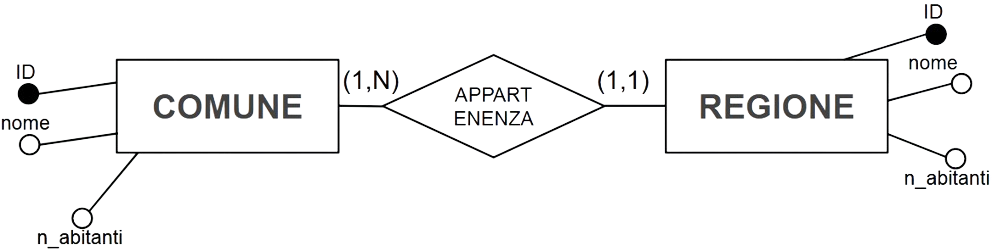
\includegraphics[width=0.7\textwidth]{img/i1.png}
    \end{figure}}
    \only<3>{\begin{figure}[h]
        \centering
        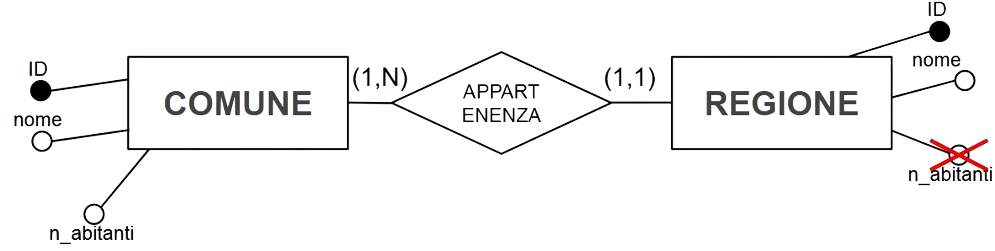
\includegraphics[width=0.7\textwidth]{img/i2.png}
    \end{figure}}
    \only<4>{\begin{figure}[h]
        \centering
        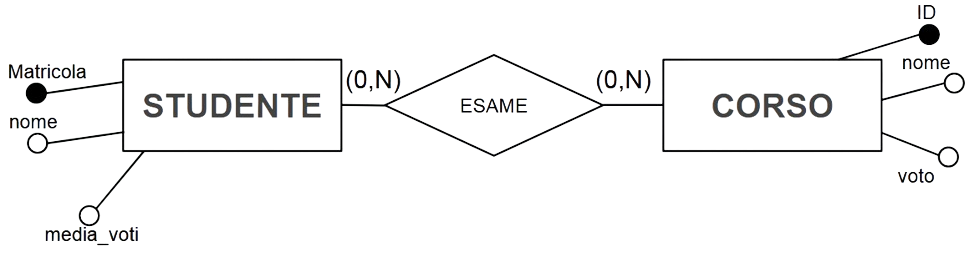
\includegraphics[width=0.7\textwidth]{img/i3.png}
    \end{figure}}
    \only<5>{\begin{figure}[h]
        \centering
        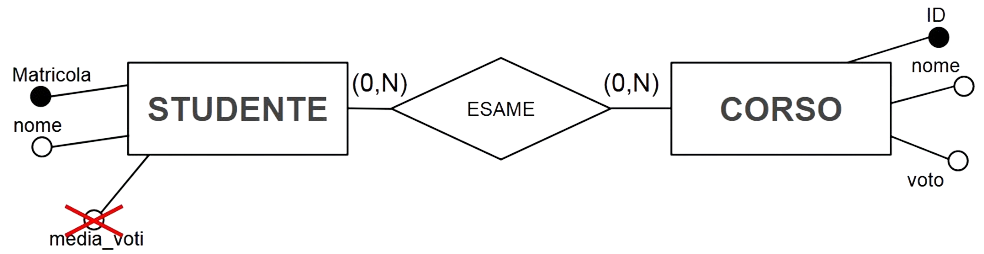
\includegraphics[width=0.7\textwidth]{img/i4.png}
    \end{figure}}
\end{frame}
%
\begin{frame}{Ristrutturazion: Fase 2}
\textbf{2) Partizionamento/accorpamento di entit\`a e associazioni}
\\\vspace{2em}
Gli accessi ad una entit\`a possono essere ridotti separando o raggruppando degli attributi.
\begin{figure}[h]
        \centering
        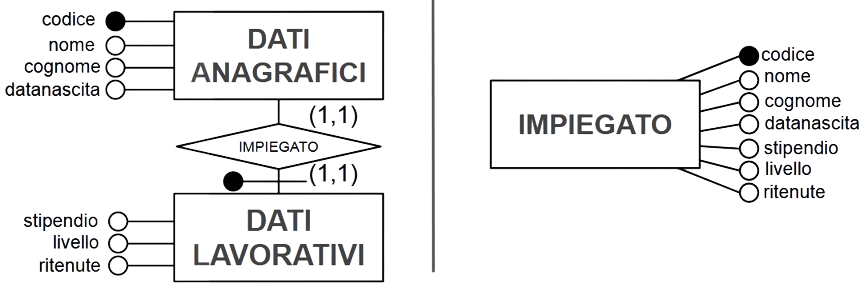
\includegraphics[width=0.8\textwidth]{img/i5.png}
    \end{figure}
\end{frame}
%
\begin{frame}{Ristrutturazion: Fase 3}
\textbf{3) Eliminazione delle generalizzazioni}
\\\vspace{2em}
Il modello logico del DB non permette la presenza di generalizzazioni, vanno quindi eliminate. Ci sono 3 diversi metodi di eliminazione e vanno scelti in base alle esigenze.
\begin{figure}[h]
        \centering
        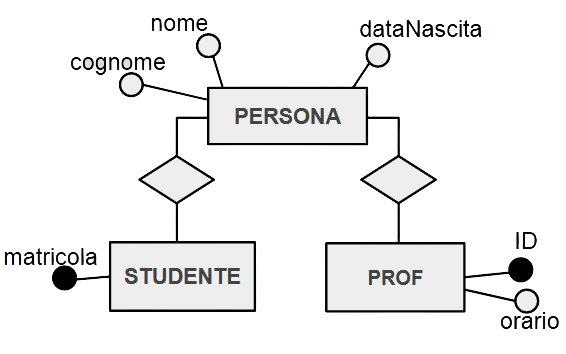
\includegraphics[width=0.5\textwidth]{img/i6.png}
    \end{figure}
\end{frame}
%
\begin{frame}{Ristrutturazione}
\textbf{3) Eliminazione delle generalizzazioni}
\\\vspace{2em}
\begin{center}
    \textbf{MANTENIMENTO DELLE ENTIT\`A CON ASSOCIAZIONI}
\end{center}
\begin{columns}
        \begin{column}{0.5\textwidth}
            \begin{figure}[h]
        \centering
        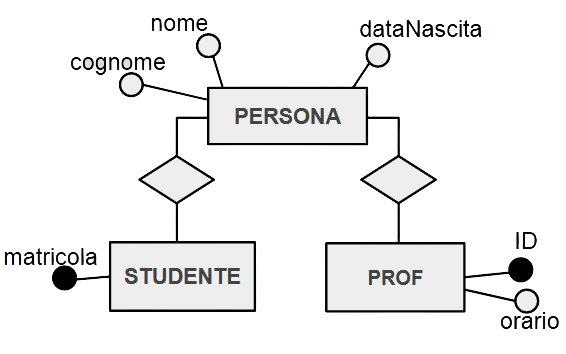
\includegraphics[width=1\textwidth]{img/i6.png}
    \end{figure}
        \end{column}
        \begin{column}{0.5\textwidth}
            \begin{figure}[h]
        \centering
        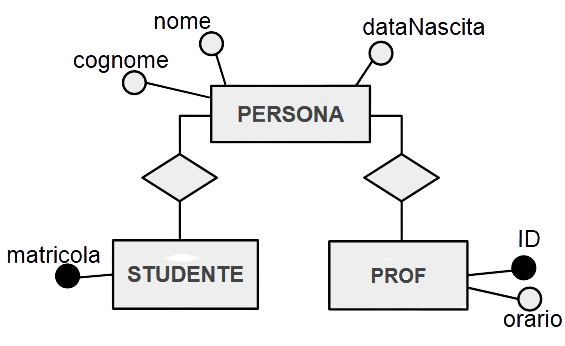
\includegraphics[width=1\textwidth]{img/i7.png}
    \end{figure}
        \end{column}
    \end{columns}
\end{frame} 
%
\begin{frame}{Ristrutturazion: Fase 3}
\textbf{3) Eliminazione delle generalizzazioni}
\\\vspace{2em}
\begin{center}
    \textbf{COLLASSO VERSO L`ALTO}
\end{center}
\begin{columns}
        \begin{column}{0.5\textwidth}
            \begin{figure}[h]
        \centering
        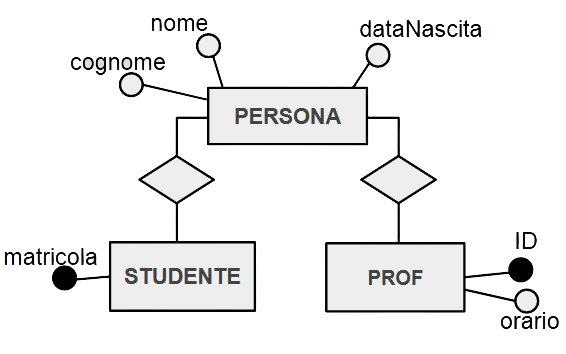
\includegraphics[width=1\textwidth]{img/i6.png}
    \end{figure}
        \end{column}
        \begin{column}{0.5\textwidth}
            \begin{figure}[h]
        \centering
        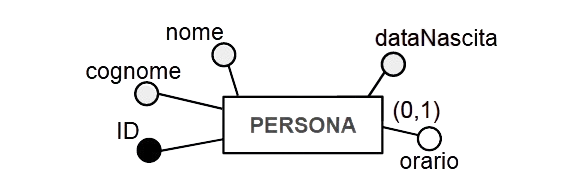
\includegraphics[width=1\textwidth]{img/i8.png}
    \end{figure}
        \end{column}
    \end{columns}
\end{frame}
%
\begin{frame}{Ristrutturazion: Fase 3}
\textbf{3) Eliminazione delle generalizzazioni}
\\\vspace{2em}
\begin{center}
    \textbf{COLLASSO VERSO IL BASSO}
\end{center}
\begin{columns}
        \begin{column}{0.5\textwidth}
            \begin{figure}[h]
        \centering
        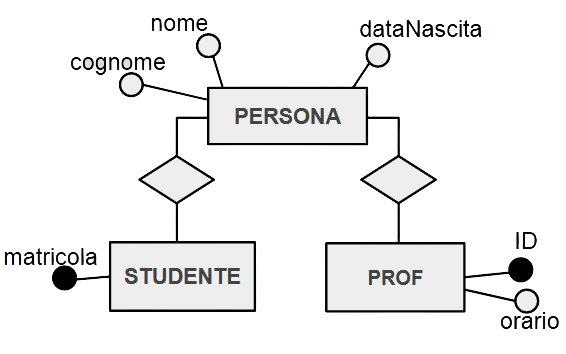
\includegraphics[width=1\textwidth]{img/i6.png}
    \end{figure}
        \end{column}
        \begin{column}{0.5\textwidth}
            \begin{figure}[h]
        \centering
        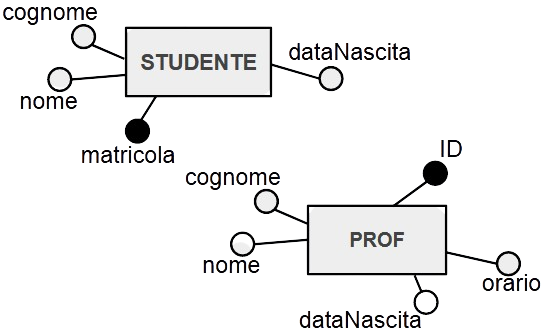
\includegraphics[width=0.9\textwidth]{img/i9.png}
    \end{figure}
        \end{column}
    \end{columns}
\end{frame}
%
\begin{frame}{Ristrutturazion: Fase 4}
\vspace{-3cm}
\textbf{4) scelta degli identificatori primari}
\\\vspace{2em}
Le chiavi primarie devono essere non nulle e non esterne. Sono da preferire chiavi non composte o almeno composte da meno attributi possibile.
\end{frame}
%
\begin{frame}{Ristrutturazion: Fase 5}
\textbf{5) Normalizzazione degli attributi}
\\\vspace{2em}
Gli attributi composti devono essere rimossi.
\begin{columns}
        \begin{column}{0.5\textwidth}
            \begin{figure}[h]
        \centering
        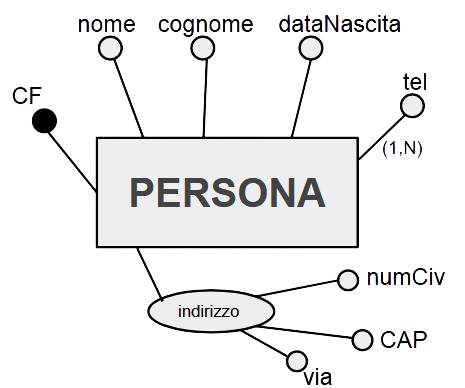
\includegraphics[width=0.75\textwidth]{img/i10.png}
    \end{figure}
        \end{column}
        \begin{column}{0.5\textwidth}
        \uncover<2->{\only<2>{\begin{figure}[h]
        \centering
        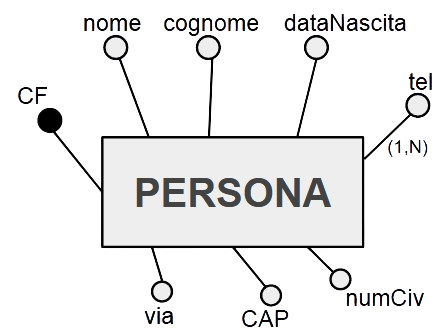
\includegraphics[width=0.8\textwidth]{img/i11.png}
    \end{figure}}
    \only<3>{\begin{figure}[h]
        \centering
        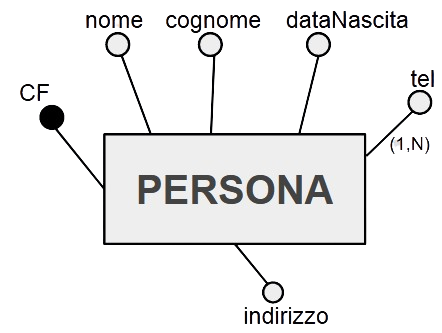
\includegraphics[width=0.8\textwidth]{img/i12.png}
    \end{figure}}}
        \end{column}
    \end{columns}
\end{frame}
%
\begin{frame}{Ristrutturazion: Fase 5}
\textbf{5) Normalizzazione degli attributi}
\\\vspace{2em}
Gli attributi con cardinalit\`a devono essere trasformati in entit\`a
\begin{columns}
        \begin{column}{0.5\textwidth}
            \begin{figure}[h]
        \centering
        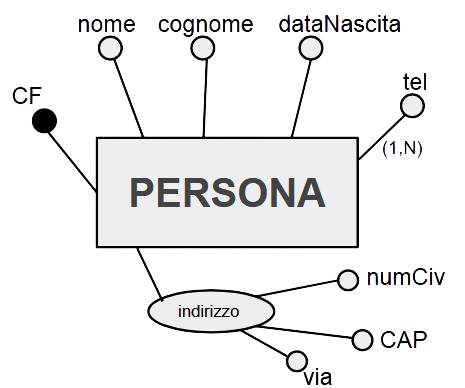
\includegraphics[width=0.75\textwidth]{img/i10.png}
    \end{figure}
        \end{column}
        \begin{column}{0.5\textwidth}
        \uncover<2->{\begin{figure}[h]
        \centering
        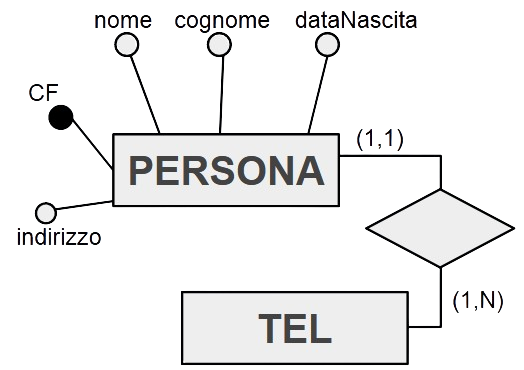
\includegraphics[width=0.8\textwidth]{img/i13.png}
    \end{figure}}
        \end{column}
    \end{columns}
\end{frame}
%
\begin{frame}{Traduzione}
\textbf{associazione uno-a-uno}
    \begin{figure}[h]
        \centering
        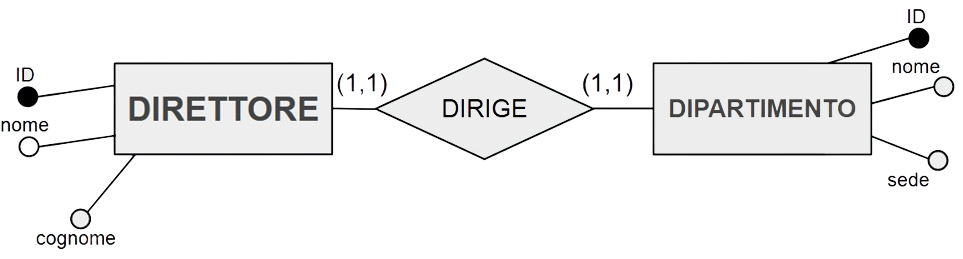
\includegraphics[width=0.8  \textwidth]{img/i14.png}
    \end{figure}
\begin{center}
\begin{tikzpicture}
    \node[draw=black, thick, inner sep=5pt, scale=0.9] {
        \begin{tabular}{ll}
            \textbf{DIRETTORE} & (\underline{ID}$^{\#}$, nome, cognome) \\
            \textbf{DIPARTIMENTO} & (\underline{ID}, nome, sede, direttore$^{\#}$)
        \end{tabular}
    };
\end{tikzpicture}
\vspace{0.3cm}

\uncover<2->{\begin{tikzpicture}
    \node[draw=black, thick, inner sep=5pt,scale = 0.9] {
        \begin{tabular}{ll}
            \textbf{DIRETTORE} & (\underline{ID}, nome, cognome, dipartimento$^{\#}$) \\
            \textbf{DIPARTIMENTO} & (\underline{ID}$^{\#}$, nome, sede)
        \end{tabular}
    };
\end{tikzpicture}}
\end{center}
\end{frame}
%
\begin{frame}{Traduzione}
\textbf{associazione uno-a-uno}
    \begin{figure}[h]
        \centering
        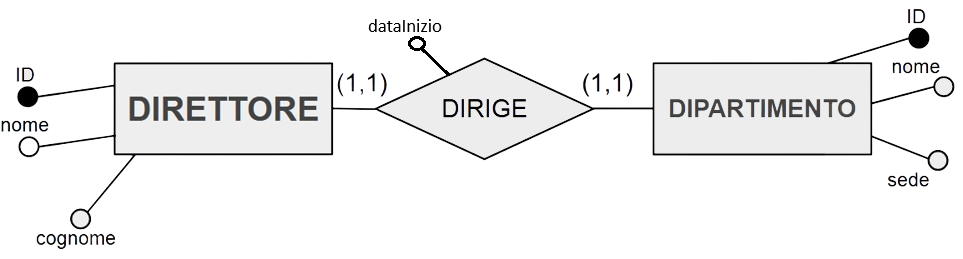
\includegraphics[width=0.8  \textwidth]{img/i14_2.png}
    \end{figure}
\begin{center}
\begin{tikzpicture}
    \node[draw=black, thick, inner sep=5pt, scale=0.9] {
        \begin{tabular}{ll}
            \textbf{DIRETTORE} & (\underline{ID}$^{\#}$, nome, cognome) \\
            \textbf{DIPARTIMENTO} & (\underline{ID}, nome, sede, dataInizio, direttore$^{\#}$)
        \end{tabular}
    };
\end{tikzpicture}
\vspace{0.3cm}

\uncover<2->{\begin{tikzpicture}
    \node[draw=black, thick, inner sep=5pt,scale = 0.9] {
        \begin{tabular}{ll}
            \textbf{DIRETTORE} & (\underline{ID}, nome, cognome, dataInizio, dipartimento$^{\#}$) \\
            \textbf{DIPARTIMENTO} & (\underline{ID}$^{\#}$, nome, sede)
        \end{tabular}
    };
\end{tikzpicture}}
\end{center}
\end{frame}
%
\begin{frame}{Traduzione}
\textbf{associazione uno-a-molti (attributo su relazione)}
    \begin{figure}[h]
        \centering
        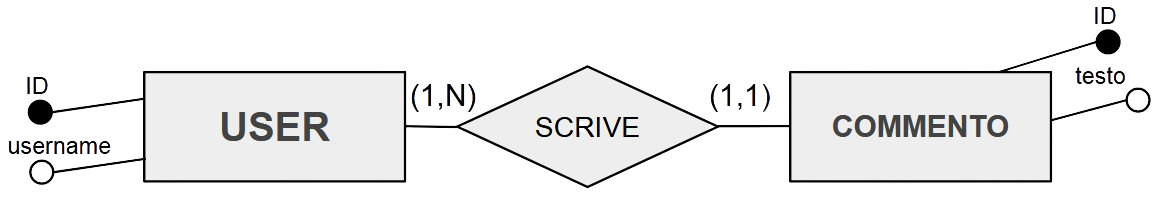
\includegraphics[width=0.8  \textwidth]{img/i15.png}
    \end{figure}
    \vspace{0.8cm}
\uncover<2->{\begin{center}
    \begin{tikzpicture}
    \node[draw=black, thick, inner sep=5pt, scale=0.9] {
        \begin{tabular}{ll}
            \textbf{USER} & (\underline{ID}$^{\#}$, username) \\
            \textbf{COMMENTO} & (\underline{ID}, testo, user$^{\#}$)
        \end{tabular}
    };
\end{tikzpicture}
\end{center}}
\end{frame}
%
\begin{frame}{Traduzione}
\textbf{associazione uno-a-molti}
    \begin{figure}[h]
        \centering
        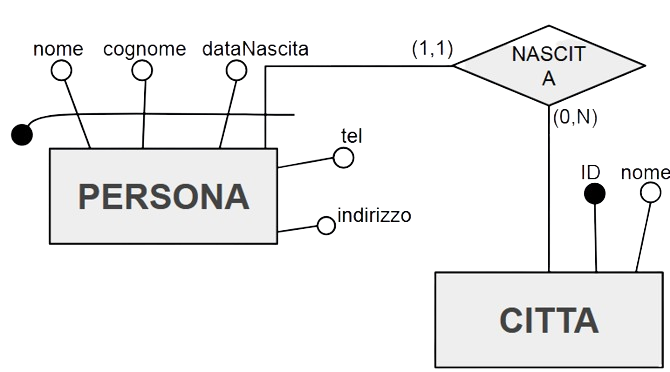
\includegraphics[width=0.5  \textwidth]{img/i16.png}
    \end{figure}
    \vspace{0.5cm}
\uncover<2->{
\begin{center}\only<2>{
    \begin{tikzpicture}
    \node[draw=black, thick, inner sep=5pt, scale=0.9] {
        \begin{tabular}{ll}
            \textbf{PERSONA} & (\underline{nome}, \underline{cognome}, \underline{dataNascita}, \underline{citta}$^{\#}$, tel. indirizzo) \\
            \textbf{CITTA} & (\underline{ID}$^{\#}$, nome)
        \end{tabular}
    };
\end{tikzpicture}}
\only<3>{
    \begin{tikzpicture}
    \node[draw=black, thick, inner sep=5pt, scale=0.9] {
        \begin{tabular}{ll}
            \textbf{PERSONA} & (\underline{nome}, \underline{cognome}, \underline{dataNascita}, \underline{CP}$^{\#}$, \underline{nomeCitta}$^{*}$, tel. indirizzo) \\
            \textbf{CITTA} & (\underline{CodicePostale}$^{\#}$, \underline{nome}$^{*}$)
        \end{tabular}
    };
\end{tikzpicture}}
\end{center}}
\end{frame}
%
\begin{frame}{Traduzione}
\textbf{associazione molti-a-molti}
\begin{figure}[h]
        \centering
        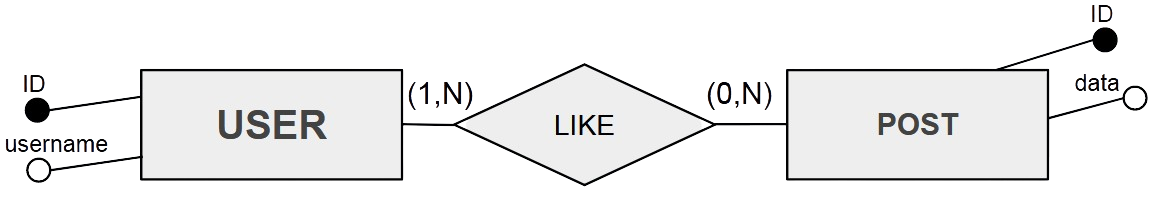
\includegraphics[width=1  \textwidth]{img/i17.png}
\end{figure}
\vspace{0.8cm}
\begin{center}
\uncover<2->{
\begin{tikzpicture}
    \node[draw=black, thick, inner sep=5pt, scale=0.9] {
        \begin{tabular}{ll}
            \textbf{USER} & (\underline{ID}$^{\#}$, username) \\
            \textbf{POST}& (\underline{ID}$^*$, data)\\
            \textbf{LIKE} & (\underline{USER}$^{\#}$, \underline{POST}$^{*}$)
        \end{tabular}
    };
\end{tikzpicture}}
\end{center}
\end{frame}
%
\begin{frame}{Traduzione}
\textbf{associazione molti-a-molti(ricorsiva)}
\begin{figure}[h]
        \centering
        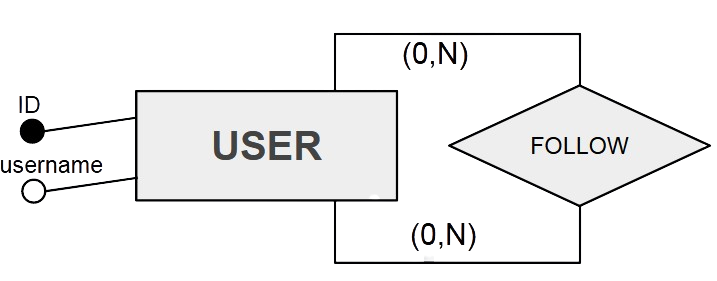
\includegraphics[width=0.7  \textwidth]{img/i18.png}
\end{figure}
\vspace{0.5cm}
\begin{center}
\uncover<2->{\begin{tikzpicture}
    \node[draw=black, thick, inner sep=5pt, scale=0.9] {
        \begin{tabular}{ll}
            \textbf{USER} & (\underline{ID}$^{\#*}$, username) \\
            \textbf{FOLLOW}& (\underline{IDfollower}$^\#$, \underline{IDfollowed}$^*$)\\
        \end{tabular}
    };
\end{tikzpicture}}
\end{center}
\end{frame}
%
\section{Conclusioni}

\begin{frame}{Domande?}
    \begin{figure}
\centering
    
\includegraphics[width=0.75\textwidth]{../img/questions.jpg}
\end{figure}
\end{frame}

\begin{frame}{Fine}
    \centering
    \huge Grazie dell'attenzione!
\end{frame}

\end{document}